\documentclass[10pt,openany]{book}

% 基本内容
\newcommand{\mytitleen}{CAD cook-book}
\newcommand{\mytitle}{CAD口袋书}
\newcommand{\myauthor}{清华大学电子系学培部}
\newcommand{\mycp}{面向《电子电路与系统基础》（A）的电路仿真参考}
\newcommand{\sampletext}{}
% \def\freefont{} % 使用免费商业字体
\def\costomizetitlepage{} % 使用自定义扉页titlepage.tex
\def\footinfo{} % 将页码等信息放在页脚，不启用则放在页眉
\def\tutor{}
% \def\bleed{} % 出血
% \def\startonchapter{} % 以chapter作为一级标题，不启用则以part作为一级

% 字体配置
\ifdefined\freefont
    \usepackage{fontspec}
    \setmainfont{EB Garamond}
    \newfontfamily\sbien{EB Garamond SemiBold Italic}
    \newfontfamily\pagenfont{EB Garamond Medium Italic}
    \newfontfamily\prenotefont{EB Garamond Medium}
    \newfontfamily\cpfont{EB Garamond Italic}

    \newfontfamily\normal{Source Han Serif CN}
    \newfontfamily\semib{Source Han Serif CN SemiBold} % 小标宋
    \newfontfamily\bold{Source Han Serif CN Bold} % 大标宋
    \newfontfamily\heavy{Source Han Serif CN Heavy} % 粗宋

    \newfontfamily\shusongen{FZShuSong-Z01S} % 书宋
    \newfontfamily\kaitien{FZKai-Z03S} % 楷体
    \newfontfamily\heitien{FZHei-B01S} % 黑体

    \newfontfamily\titlefonten{EB Garamond 12 Italic}[LetterSpace=1]
    \newfontfamily\namefont{Scriptina}[LetterSpace=5]

    \usepackage[fontset=none]{ctex}
    \setCJKmainfont{Source Han Serif CN}[BoldFont={Source Han Serif CN SemiBold}, ItalicFont=FZKai-Z03]

    \newCJKfontfamily\songti{Source Han Serif CN}
    \newCJKfontfamily\xbsong{Source Han Serif CN SemiBold} % 小标宋
    \newCJKfontfamily\dbsong{Source Han Serif CN Bold} % 大标宋
    \newCJKfontfamily\cusong{Source Han Serif CN Heavy} % 粗宋

    \newCJKfontfamily\shusong{FZShuSong-Z01}[ItalicFont=FZKai-Z03] % 书宋
    \newCJKfontfamily\fangsong{FZFangSong-Z02} % 仿宋
    \newCJKfontfamily\heiti{FZHei-B01} % 黑体
    \newCJKfontfamily\kaiti{FZKai-Z03} % 楷体

    \newcommand{\titlefont}{\titlefonten\fangsong}
    \newcommand{\signfont}{\writing}

    \newcommand{\tocmain}{\dbsong}
    \newcommand{\tocpart}{\xbsong\sbien}
    \newcommand{\tocchapter}{\xbsong}
    \newcommand{\tocchaplabel}{\itshape}
    \newcommand{\tocpage}{\pagenfont}

    \newcommand{\partfont}{\dbsong\bold}
    \newcommand{\chapterfont}{\dbsong\bold}
    \newcommand{\sectionfont}{\xbsong\semib}
    \newcommand{\subsectionfont}{\songti\normal}
    \newcommand{\pagenumberfont}{\tocpage}
    \newcommand{\headfont}{\fangsong}
    \newcommand{\quotefont}{\itshape}
    \newcommand{\writing}{\rmfamily\xbsong}
    \newcommand{\spellfont}{\quotefont}
    \newcommand{\dotfont}{\shusong}
    \newcommand{\tempfont}{\normal}
\else
    \usepackage{ctex}
    \newcommand{\prenotefont}{\rmfamily}
    \newcommand{\titlefont}{}
    \newcommand{\signfont}{\ttfamily}
    \newcommand{\cpfont}{\ttfamily}

    \newcommand{\tocmain}{\bfseries}
    \newcommand{\tocpart}{\bfseries}
    \newcommand{\tocchapter}{\itshape}
    \newcommand{\tocchaplabel}{\itshape}
    \newcommand{\tocpage}{\ttfamily}

    \newcommand{\partfont}{\bfseries\itshape}
    \newcommand{\chapterfont}{\bfseries}
    \newcommand{\sectionfont}{\bfseries}
    \newcommand{\subsectionfont}{\sffamily}
    \newcommand{\pagenumberfont}{\tocpage}
    \newcommand{\headfont}{\ttfamily}
    \newcommand{\quotefont}{\itshape}
    \newcommand{\writing}{\rmfamily\ttfamily}
    \newcommand{\spellfont}{\quotefont}
    \newcommand{\dotfont}{\rmfamily}
    \newcommand{\tempfont}{\rmfamily}
\fi


% 首段缩进
\usepackage{indentfirst}

% 启用并隐藏超链接
\usepackage{hyperref}
\hypersetup{hidelinks}

% 页面配置
\usepackage{geometry}
% 主布局
\newlength{\pw}
\newlength{\ph}
% A5 148*210
\setlength{\pw}{148mm}
\setlength{\ph}{210mm}

\newlength{\bleedlen}
\setlength{\bleedlen}{0mm}

\newlength{\ptop}
\newlength{\pbottom}
\newlength{\pinner}
\newlength{\pouter}
\newlength{\phsep}
\newlength{\pfskip}

\setlength{\ptop}{17mm}
\setlength{\pbottom}{23mm}
\setlength{\pinner}{22mm}
\setlength{\pouter}{13.5mm}
\setlength{\phsep}{7mm}
\setlength{\pfskip}{12mm}
% 目录页布局
\newcommand{\tocgeo}{}
\ifdefined\bleed
    \addtolength{\bleedlen}{3mm}
    \addtolength{\pw}{\bleedlen}
    \addtolength{\pw}{\bleedlen}
    \addtolength{\ph}{\bleedlen}
    \addtolength{\ph}{\bleedlen}
    \addtolength{\ptop}{\bleedlen}
    \addtolength{\pbottom}{\bleedlen}
    \addtolength{\pinner}{\bleedlen}
    \addtolength{\pouter}{\bleedlen}
    \renewcommand{\tocgeo}{\newgeometry{left=40mm,right=40mm,top=\ptop,bottom=\pbottom}}
\else
    \renewcommand{\tocgeo}{\newgeometry{left=37mm,right=37mm,top=\ptop,bottom=\pbottom}}
\fi
\ifdefined\footinfo
    \geometry{
        paperwidth=\pw,
        paperheight=\ph,
        top=\ptop,
        bottom=\pbottom,
        outer=\pouter,
        inner=\pinner,
        footskip=\pfskip,
    }
\else
    \geometry{
        paperwidth=\pw,
        paperheight=\ph,
        top=\pbottom,
        bottom=\ptop,
        outer=\pouter,
        inner=\pinner,
        headsep=\phsep,
    }
\fi

% 空白页
\newcommand{\blankpage}{
    \newpage
    \makebox{}
    \thispagestyle{empty}
    \newpage
}

% 空白段
\newcommand{\blankline}{
    ~\
}

% 目录
% 目录参数
\counterwithout{section}{chapter}
\counterwithout{subsection}{section}
% 目录格式
\usepackage{titletoc}
% 章节符号
\newcommand{\myss}{\textit{\textbf{\S}}}
% 目录内标题格式
\ifdefined\startonchapter
    % 目录标题
    \renewcommand{\contentsname}{
        {\hspace{10mm}}目\hspace{0.75em}录
    }
    \titlecontents{chapter}
    [0em]
    {\vspace{2em}\Large\tocchapter}
    {\makebox[10mm][l]{\myss\hspace{0.1em}\large\uppercase\expandafter{\romannumeral\thecontentslabel}}}
    {}
    {\hspace{4mm}\tocpage\large\contentspage}[\vspace{1.6em}]

    \titlecontents{section}
    [21mm]
    {\tocsection}
    {\tocsectlabel Ch \hspace{0.1em}\makebox[1em][c]{\thecontentslabel}}{}
    {\hspace{5mm}\tocpage\contentspage}[\vspace{0.1em}]
\else
    % 目录标题
    \renewcommand{\contentsname}{
    {\hfill}目\hspace{0.75em}录{\hfill}
    \vspace{7mm}
    }
    \titlecontents{part}
    [0em]
    {\Large\tocpart}
    {}
    {}
    {\hfill\pagenumberfont\contentspage}[\vspace{1.6em}]

    \titlecontents{chapter}
    [2em]
    {\tocchapter}
    {\thecontentslabel\quad}
    {}
    {\hfill\pagenumberfont\contentspage}[]
\fi

\makeatletter
% 页码宽度
\renewcommand{\contentspage}[1][\thecontentspage]{\hb@xt@\@pnumwidth{#1\hfil}}
\renewcommand{\@pnumwidth}{7mm}
\ifdefined\startonchapter
    % 每章重置尾注编号
    \@addtoreset{endnote}{chapter}  % Reset endnote numbering every new chapter
\else
    \@addtoreset{endnote}{part}  % Reset endnote numbering every new part
    \@addtoreset{chapter}{part}  % Reset chapter numbering every new part
\fi
\makeatother
% 每页重置脚注编号
\usepackage{footnpag}

% 正文标题格式
\usepackage{titlesec}

\ifdefined\startonchapter
    \titleformat{\chapter}{\huge\chapterfont}{}{1em}{\thispagestyle{empty}}
    \titleformat{\section}{\sectionfont}{Chapter~\thesection}{1em}{}
    \titleformat{\subsection}{\subsectionfont}{0\thesubsection}{1em}{}

    \titlespacing*{\chapter}{0em}{5em}{\chapterblank}
    \titlespacing*{\section}{2em}{1.5\baselineskip}{.5\baselineskip}
    \titlespacing*{\subsection}{2em}{.5\baselineskip}{.5\baselineskip}
\else
    \titleformat{\part}[display]{\centering\Huge\partfont}{\thepart}{1.5pc}{\thispagestyle{empty}}
    \titleformat{\chapter}{\centering\Large\chapterfont}{第\zhnumber{\thechapter}章}{1em}{}
    \titlespacing{\part}{0em}{5cm}{0em}
    \titlespacing*{\chapter}{0em}{1em}{3em}
\fi

\newcommand{\parttitle}{部名}

\usepackage{fancyhdr}
% 章标记不出现chapter和序号
\renewcommand{\chaptermark}[1]{\markboth{\MakeUppercase{#1}}{}}
% 去除页眉横线
\renewcommand{\headrulewidth}{0pt}
\ifdefined\footinfo
    \fancypagestyle{mystyle}{
        \fancyhf{}
        \fancyfoot[LE]{\pagenumberfont\thepage\quad\headfont\parttitle}
        \fancyfoot[RO]{\headfont\leftmark\quad\pagenumberfont\thepage}
    }
\else
    \fancypagestyle{mystyle}{
        \fancyhf{}
        \fancyhead[LE,RO]{\pagenumberfont\thepage}
        \fancyhead[CE]{\headfont\mytitle}
        \fancyhead[CO]{\headfont\leftmark}
    }
\fi
\fancypagestyle{plain}{
    \fancyhf{}
    \fancyfoot[LE]{\pagenumberfont\thepage\quad\headfont\parttitle}
    \fancyfoot[RO]{\pagenumberfont\thepage}
}
\usepackage{emptypage}

% 尾注
\usepackage{endnotes}
\renewcommand{\notesname}{注：}
\renewcommand{\enoteheading}{\section*{\notesname}\mbox{}\par\vskip-\baselineskip}

% 以下为非通用内容

% 故事完
\newcommand{\storyend}[1][完]{
    \blankline

    \blankline

    \hfill {\bfseries #1} \hspace{5em}

    \vfill
}

% 设置quote区中的字体
\usepackage{etoolbox}
\AtBeginEnvironment{quote}{\quotefont}

% 设置署名
\newcommand{\signature}{
    \vfill

    \hfill {\subsectionfont by\myauthor} \hspace{5em}

    \hfill {\subsectionfont 2024.08.09} \hspace{4.8em}

    \vspace{2cm}
}

% 特殊符号和字体
\newcommand{\splitdot}{\dotfont ·}

\newcommand{\spell}[1]{{\spellfont #1}}

\newcommand{\tempsymbol}{{\tempfont℃}}

\newcommand{\chsline}{\hspace{0.15em}\rule[0.35em]{1.7em}{0.03em}\hspace{0.15em}}

% 章前注的参数
\newlength{\chapterblank}
\setlength{\chapterblank}{3cm}
\newlength{\prenoteblank}
\setlength{\prenoteblank}{3em}
\newcommand{\doublelinechapter}{{\huge\vspace{-\baselineskip}}}

% 章前注
\newcommand{\prenotes}[1]{
    \vspace{2em}
    {\prenotefont #1}
    % #1
    \vspace{0.5em}
    \vspace{\prenoteblank}
}

% 扉页
\newcommand{\mytitlepage}{
    \thispagestyle{empty}
    % 封面图
    \begin{center}
        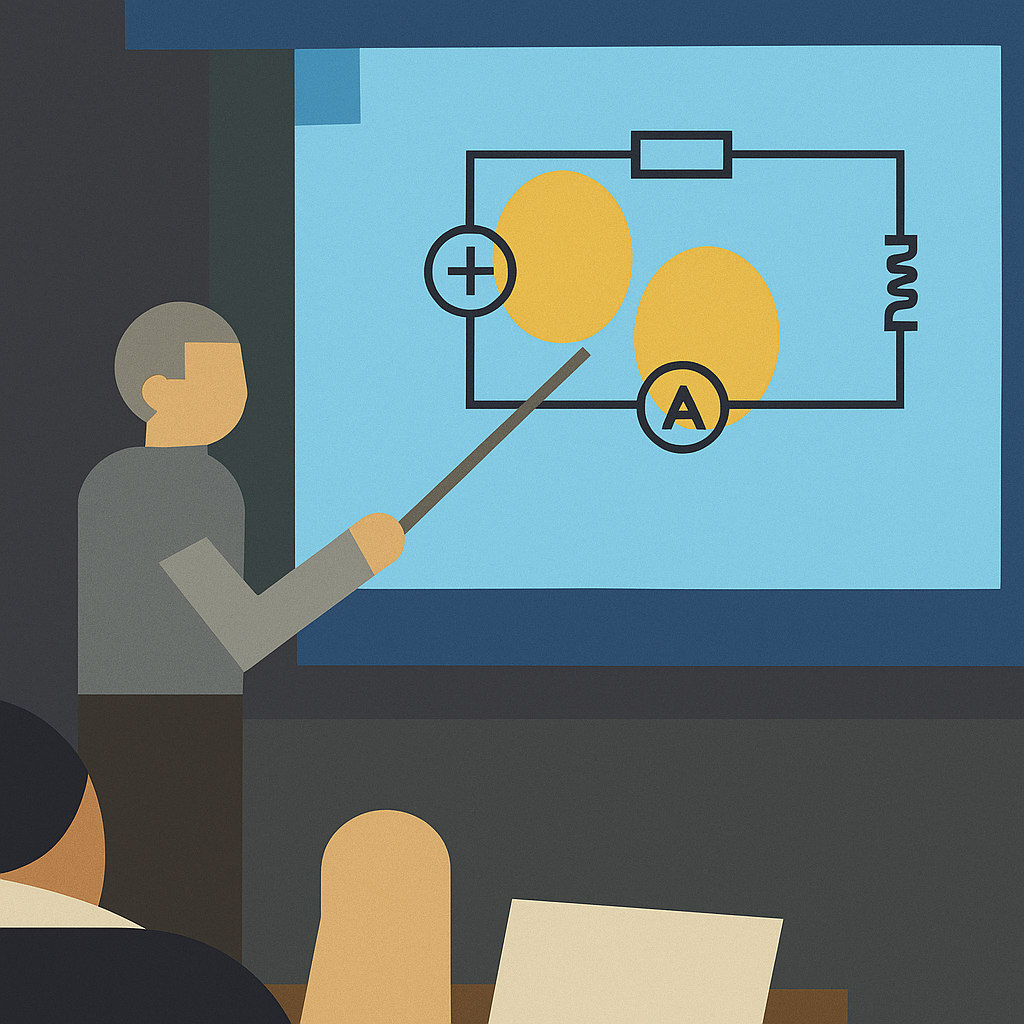
\includegraphics[width=\textwidth]{figure/cover.png}
    \end{center}

    % \vspace{-0.1cm} % 图片和标题之间留白
% 标题和logo之间留白
    \noindent
    \begin{minipage}[b]{0.68\textwidth}
        \raggedright
        \begingroup
            % \setlength{\fboxsep}{0pt}% no padding around colorbox
            % \noindent
            % \hspace*{}%
            {\setlength{\fboxsep}{1pt}\noindent\colorbox{cyan}{\makebox[\textwidth][l]{\rule{0pt}{5mm}}}}%      \hspace*{\dimexpr\hoffset+1in+\oddsidemargin\relax}%
        \endgroup
        % \RequirePackage{xcolor}
        

        {\Huge\titlefont \mytitle \par}
        \vspace{5mm}
        {\cpfont \mycp \par}
        \vspace{3mm}
        {\large\signfont BY \myauthor \par}
    \end{minipage}%
    \hfill
    \begin{minipage}[b]{0.29\textwidth}
        \raggedleft
        {\cpfont $\triangle $Created by \href{https://sora.com}{sora} \\
        \par}
        \vspace{8mm}

        % \vspace{-1em} % 调整logo垂直位置，可微调
        
\includegraphics[width=\textwidth]{figure/logo.png}
    \end{minipage}

    \vfill
}


% 尾页
\newcommand{\myendpage}{
    \newpage

    \thispagestyle{empty}

    \

    \vfill

    \begin{minipage}{100mm}

        有任何改进建议请联系：\href{mailto:jiangwt23@mails.tsinghua.edu.cn}{jiangwt23@mails.tsinghua.edu.cn}\\

        感谢您对电子系学生科协的支持！

    \end{minipage}
    \vspace{5mm}
}

% 调整行距为1.618
\usepackage{setspace}
\setstretch{1.618}
% 段距增加弹性
\setlength{\parskip}{0em plus .1\baselineskip}

% 插入图片
\usepackage{graphicx}
\usepackage{float}

\usepackage{subfiles}
\usepackage{xcolor}
\title{\mytitleen\\\mytitle}
\author{\myauthor}
\date{}

\begin{document}

\pagestyle{mystyle}

\ifdefined\costomizetitlepage
    \subfile{titlepage}
\else
    \maketitle
\fi

\clearpage

{\
    \vfill
    \thispagestyle{empty}
    \Large
    \setstretch{2}
    
    本文档由\href{https://www.eesast.com}{清华大学电子系学生科协}学培部编写和维护，旨在为学习《电子电路与系统基础》的同学提供CAD学习参考。

    ~\

    \vfill
}

\ifdefined\startonchapter
    \setcounter{tocdepth}{0}
\else
    \setcounter{tocdepth}{-1}
\fi

\tocgeo
\tableofcontents
\thispagestyle{empty}

\cleardoublepage
\setcounter{page}{1}
\restoregeometry

\ifdefined\tutor
    \section{编写教程}
本章节介绍如何使用本模板编写电子电路与系统基础的学习资料。本章节不会出现在正式分发的文件中，仅供同学学习使用。
\subsection{前期准备}
\subsubsection{安装\LaTeX{}编译环境}
在编写之前，请确保您已经安装了\LaTeX{}编译环境。具体请安装TeX Live， 同时安装VsCode并在其上安装LaTeX Workshop插件。安装后，需要将默认编译引擎更换为XeLatex。方法为：
\begin{enumerate}
  \item 打开VsCode，点击插件，点击Latex Workshop插件的设置按钮，选择“扩展设置”。
    \item 找到“{\tt Latex-workshop > Latex > Recipe: Default}" 选项并将其修改为“{\tt latexmk (xelatex)}”。
\end{enumerate}
\subsubsection{安装git}
我们将基于git进行协作。请首先在\url{https://github.com}注册一个账号，并将它发给我（江玮陶），我将将你拉进本项目的协作组。\footnote{如果由于网络问题你无法访问github，请参考\url{https://register.wallesspku.org}的解决方案。}然后请在你的电脑上安装git，具体请参考\url{https://docs.eesast.com/docs/tools/git}。对于mac用户，只需要在终端运行指令
\begin{lstlisting}[language=bash]
brew install git
\end{lstlisting}
即可安装git。安装git后，请按照如下方法配置ssh key以便于后续操作：
\begin{enumerate}
  \item 在终端中运行如下指令，生成ssh key：
\begin{lstlisting}[language=bash]
ssh-keygen -t rsa -b 4096 -C "your_email@example.com"
\end{lstlisting}
  其中请将\texttt{your\_email@example.com}替换为您在GitHub上注册的邮箱地址。
    \item 在github网站上，进入Settings页面，选择SSH and GPG keys选项卡，点击New SSH key按钮。
    \item 在Title栏中输入一个名称（例如“我的电脑”），然后将刚才生成的ssh key内容粘贴到Key栏中。ssh key内容可以通过运行如下指令获得：（其中路径可能因系统和配置不同而异，请根据实际情况修改）
\begin{lstlisting}[language=bash]
cat ~/.ssh/id_rsa.pub
\end{lstlisting}
    \item 点击Add SSH key按钮完成添加。
\end{enumerate}

\subsubsection{协作工作流}
在完成上述步骤后，您就可以开始协作编写文档了。

\noindent\emph{首次克隆项目}

在您的电脑上打开终端，运行如下指令克隆项目到本地：
\begin{lstlisting}[language=bash]
git clone git@github.com:CBDT-JWT/CAD-cookbook.git

\end{lstlisting}
\noindent\emph{日常更新与提交}

在日常编写过程中，请按照如下步骤进行更新与提交：
\begin{enumerate}
  \item 在开始编写之前，先运行如下指令拉取最新的代码：
\begin{lstlisting}[language=bash]
git pull origin master
\end{lstlisting}
    \item 在完成编写后，运行如下指令将修改添加到暂存区：
\begin{lstlisting}[language=bash]
git add .
\end{lstlisting}
    \item 运行如下指令提交修改：
\begin{lstlisting}[language=bash]
git commit -m "你的提交信息"
\end{lstlisting}
    \item 运行如下指令将修改推送到远程仓库：
\begin{lstlisting}[language=bash]
git push origin master
\end{lstlisting}
\end{enumerate}

\noindent\emph{编译文档}

如果你使用vscode中的latex workshop插件，可以使用快捷键{\tt ctrl+s} (mac 为{\tt cmd+s})直接编译文档。

\subsection{\LaTeX{}基础}
\begin{center}
    {\Huge \textbf{TBD}}
\end{center}

\subsubsection{段落格式}
每个chapter文件应当独立作为一个{\tt section}, 即在段落开头使用
\begin{lstlisting}[language=TeX]
\section{章节标题}
\end{lstlisting}
来定义章节标题。章节内可以使用{\tt subsection}和{\tt subsubsection}来定义子章节。每个自然段前后应当空一行，段和图片之间也要空一行。

\subsubsection{数学公式}
数学公式可以使用美元符号{\tt \$}来包裹行内公式，例如：{\tt \$E=mc\^{}2\$}会渲染为$E=mc^2$。行间公式可以使用{\tt \$\$ ... \$\$}来包裹，例如：
\begin{lstlisting}[language=TeX]
$$
\begin{cases}
\nabla \cdot \mathbf{E} = \frac {\rho} {\varepsilon_0} \\
\nabla \cdot \mathbf{B} = 0 \\
\nabla \times \mathbf{E} = - \frac {\partial \mathbf{B}} {\partial t} \\
\nabla \times \mathbf{B} = \mu_0 \mathbf{J} + \mu_0 \varepsilon_0 \frac {\partial \mathbf{E}} {\partial t}
\end{cases}
$$
\end{lstlisting}

会渲染为：
$$
\begin{cases}
\nabla \cdot \mathbf{E} = \frac {\rho} {\varepsilon_0} \\
\nabla \cdot \mathbf{B} = 0 \\ 
\nabla \times \mathbf{E} = - \frac {\partial \mathbf{B}} {\partial t} \\
\nabla \times \mathbf{B} = \mu_0 \mathbf{J} + \mu_0 \varepsilon_0 \frac {\partial \mathbf{E}} {\partial t}
\end{cases}
$$

常用的数学符号可以参考\url{https://zhuanlan.zhihu.com/p/472919794}。

\subsubsection{表格}
表格可以使用{\tt table}环境来创建，例如：
\begin{lstlisting}[language=TeX]
\begin{table}[htbp]
    \centering
    \caption{示例表格} %表格标题
    \label{tab:example} %表格标签，方便引用
    \begin{tabular}{|l|c|r|} %这里l表示左对齐，c表示居中，r表示右对齐
    \toprule %表格顶部横线
    Header 1 & Header 2 & Header 3 \\
    \midrule %表格中部横线
    Cell 1 & Cell 2 & Cell 3 \\
    Cell 4 & Cell 5 & Cell 6 \\
    \bottomrule %表格底部横线
    \end{tabular}
\end{table}
\end{lstlisting}
会渲染为：

\begin{table}[htbp]
    \centering
    \caption{示例表格}
    \label{tab:example}
\begin{tabular}{l|c r} %这里l表示左对齐，c表示居中，r表示右对齐

\toprule %表格顶部横线
Header 1 & Header 2 & Header 3 \\
\midrule %表格中部横线
Cell 1 & Cell 2 & Cell 3 \\
Cell 4 & Cell 5 & Cell 6 \\
\bottomrule %表格底部横线
\end{tabular}
\end{table}

可以使用{\tt \textbackslash ref\{tab:example\}}的方式在正文中引用表格，例如“如表\ref{tab:example}所示”。在实际使用中，可以使用\url{https://www.tablesgenerator.com}方便地制作表格。

\subsubsection{插入图片}
图片可以使用{\tt figure}环境来插入，例如：
\begin{lstlisting}[language=TeX]
\begin{figure}[htbp]
    \centering
    
\includegraphics[width=0.5\textwidth]{chapters/figure/example.png} %插入图片，width参数控制图片宽度，chapters/figure/example.png为图片路径
    \caption{示例图片} %图片标题
    \label{fig:example} %图片标签，方便引用
\end{figure}
\end{lstlisting}

会渲染为图\ref{fig:example1}和\ref{fig:example2}所示。

\begin{figure}[htbp]
    \centering
    
\includegraphics[width=0.5\textwidth]{chapters/figure/example.png}
    \caption{示例图片}
    \label{fig:example}
\end{figure}
可以使用{\tt \textbackslash ref\{fig:example\}}的方式在正文中引用图片，例如“如图\ref{fig:example}所示”。请将图片文件放置在项目的{\tt figure}文件夹中。如果想要并列多张图片，可以使用minipage环境，例如：
\begin{lstlisting}[language=TeX]
\begin{figure}[htbp]
    \centering
    \begin{minipage}{0.45\textwidth}% 设置图片宽度为文本宽度的45%
        \centering
        
\includegraphics[width=.9\textwidth]{chapters/figure/example1.jpeg}
        \caption{示例图片1}
        \label{fig:example1}
    \end{minipage}
    \hfill
    \begin{minipage}{0.45\textwidth}
        \centering
        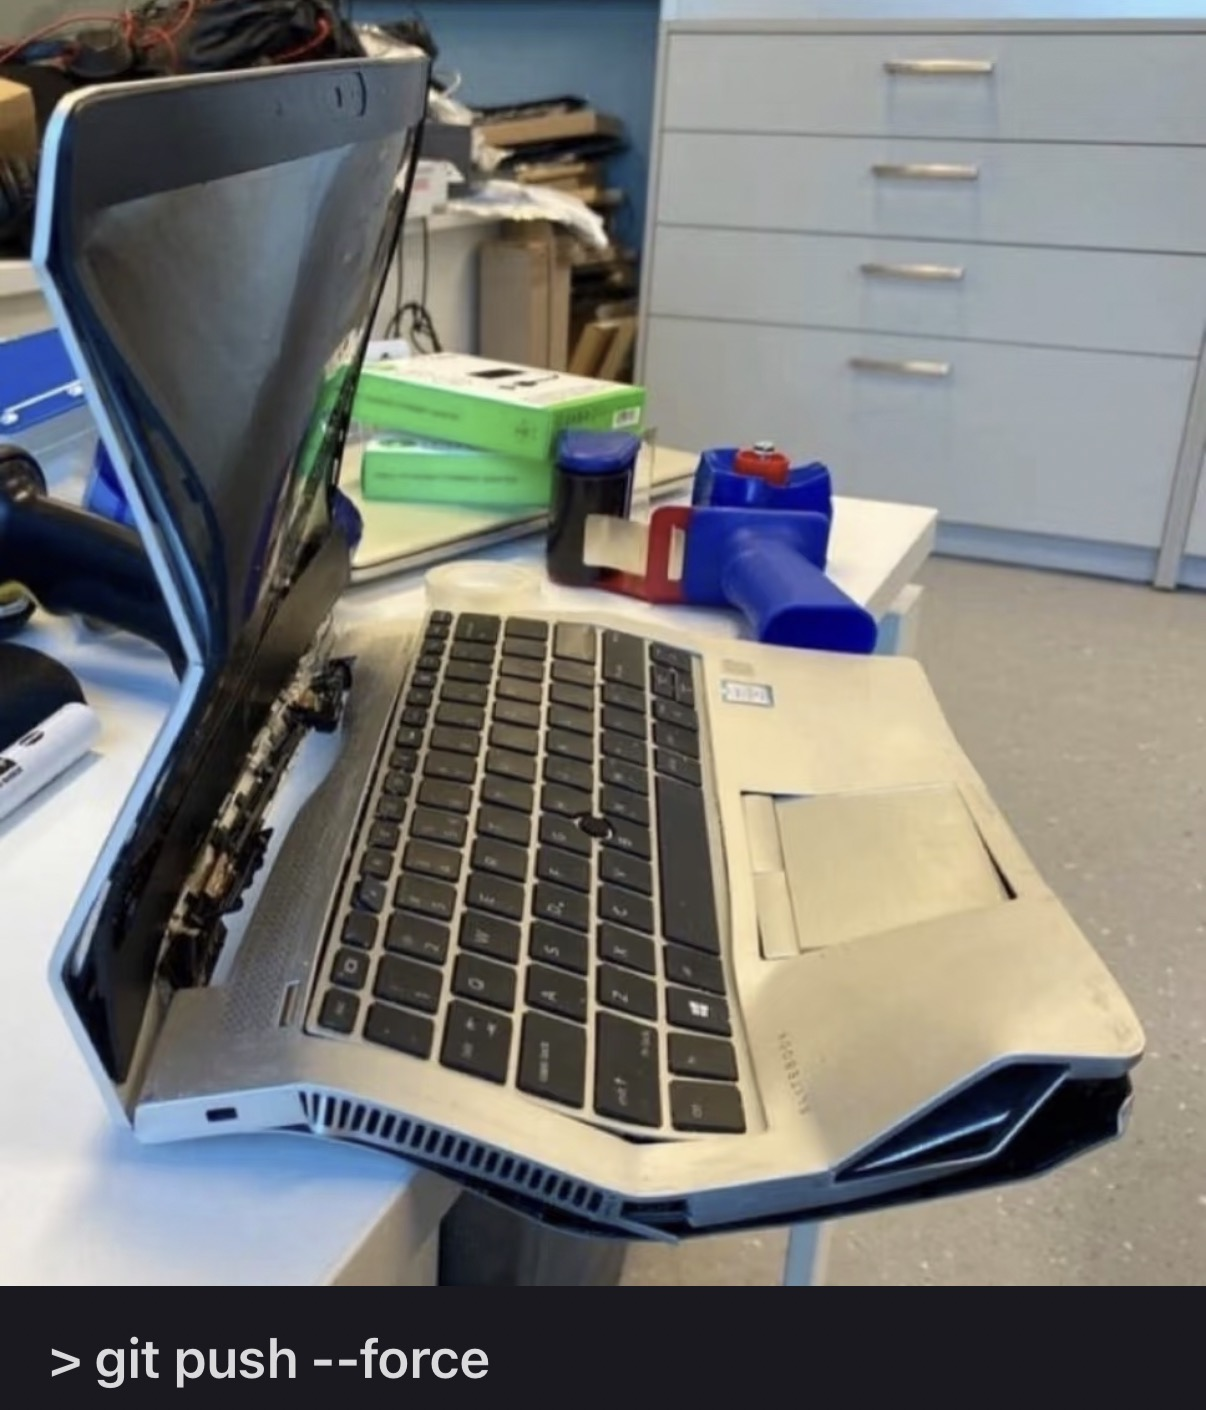
\includegraphics[width=.9\textwidth]{chapters/figure/example2.jpeg}
        \caption{示例图片2}
        \label{fig:example2}
    \end{minipage}
\end{figure}
\end{lstlisting}
会渲染为：

\begin{figure}[htbp]
    \centering
    \begin{minipage}{0.45\textwidth}
        \centering
        
\includegraphics[width=\textwidth]{chapters/figure/example1.jpeg}
        \caption{示例图片1}
        \label{fig:example1}
    \end{minipage}
    \hfill
    \begin{minipage}{0.45\textwidth}
        \centering
        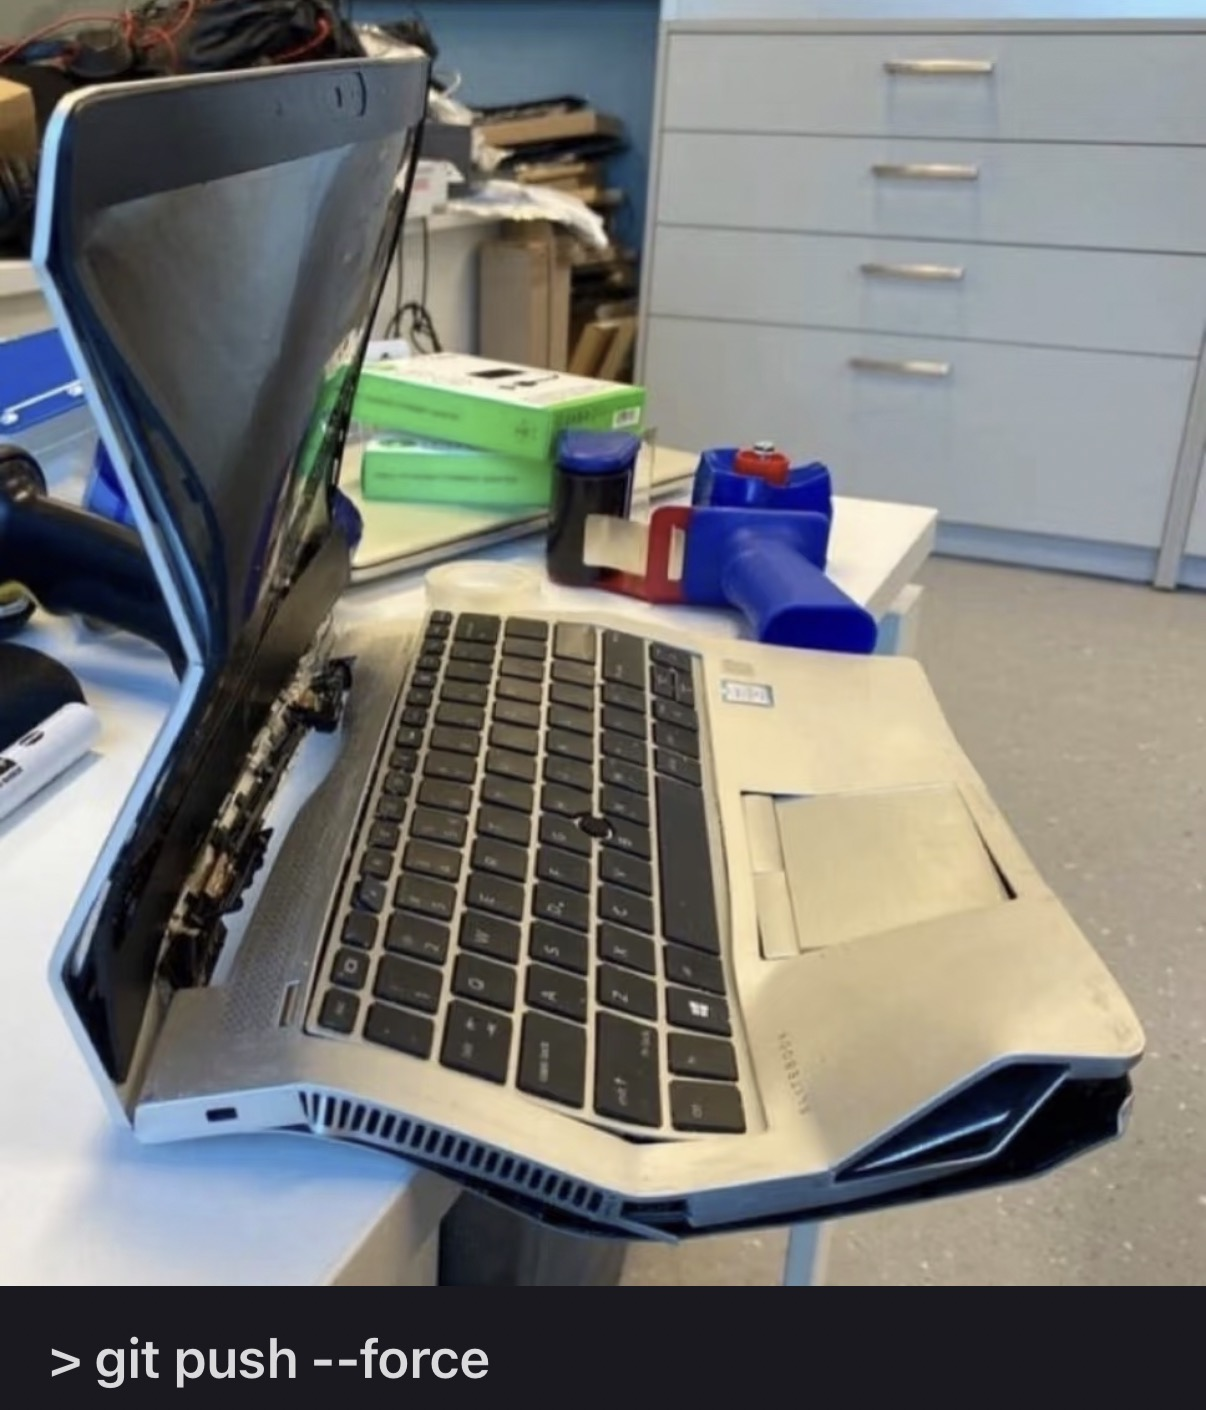
\includegraphics[width=\textwidth]{chapters/figure/example2.jpeg}
        \caption{示例图片2}
        \label{fig:example2}
    \end{minipage}
\end{figure}

\noindent\emph{电路图绘制}\quad 为了统一，我们采用circuitikz宏包绘制电路图。具体使用方法请参考\url{https://www.jiangwt.org/docs-html/documents/circuitikz/}。下面是一个简单的例子：
\begin{lstlisting}[language=TeX]
\begin{figure}[htbp]
    \centering
    \resizebox{0.6\textwidth}{!}{%
    \begin{circuitikz}
    \tikzstyle{every node}=[font=\LARGE]
    \draw (3.25,10) to[european resistor,l={ \LARGE $R_s$}] (5.5,10);
    \draw (9.25,9) to[Tnpn, transistors/scale=1.19] (9.25,11);
    \draw (5.5,10) to[C] (7.5,10);
    \node at (7.5,10) [circ] {};
    \draw (7.5,10) to[european resistor,l={ \LARGE $R_{B1}$}] (7.5,12.5);
    \draw (7.5,7.5) to[european resistor,l={ \LARGE $R_{B2}$}] (7.5,10);
    \draw (7.5,10) to[short] (8.25,10);

    \draw (7.5,7.5) to (7.5,7.25) node[ground]{};
    \draw (9.25,9) to[european resistor,l={ \LARGE $R_E$}] (9.25,7);
    \draw (9.25,7) to (9.25,6.75) node[ground]{};
    \draw (9.25,11) to[european resistor,l={ \LARGE $R_C$}] (9.25,13.25);
    \draw (8.75,13.25) to[short] (9.75,13.25);
    \draw (7,12.5) to[short] (8,12.5);
    \draw (3.25,10) to[american voltage source] (3.25,8.5);
    \draw (3.25,8.5) to (3.25,8.25) node[ground]{};
    \draw (9.25,10.75) to[C] (11.25,10.75);
    \draw (11.25,10.75) to[european resistor,l={ \LARGE $R_L$}] (11.25,8);
    \draw (11.25,10.75) to[short, -o] (12,10.75) ;

    \draw (11.25,8.75) to (11.25,8.5) node[ground]{};
    \end{circuitikz}
    }%
    \caption{样例电路}
    \label{fig: example-circuit}
\end{figure}
\end{lstlisting}


\begin{figure}[h!]
    \centering
    \resizebox{0.6\textwidth}{!}{%
    \begin{circuitikz}
    \tikzstyle{every node}=[font=\LARGE]
    \draw (3.25,10) to[european resistor,l={ \LARGE $R_s$}] (5.5,10);
    \draw (9.25,9) to[Tnpn, transistors/scale=1.19] (9.25,11);
    \draw (5.5,10) to[C] (7.5,10);
    \node at (7.5,10) [circ] {};
    \draw (7.5,10) to[european resistor,l={ \LARGE $R_{B1}$}] (7.5,12.5);
    \draw (7.5,7.5) to[european resistor,l={ \LARGE $R_{B2}$}] (7.5,10);
    \draw (7.5,10) to[short] (8.25,10);

    \draw (7.5,7.5) to (7.5,7.25) node[ground]{};
    \draw (9.25,9) to[european resistor,l={ \LARGE $R_E$}] (9.25,7);
    \draw (9.25,7) to (9.25,6.75) node[ground]{};
    \draw (9.25,11) to[european resistor,l={ \LARGE $R_C$}] (9.25,13.25);
    \draw (8.75,13.25) to[short] (9.75,13.25);
    \draw (7,12.5) to[short] (8,12.5);
    \draw (3.25,10) to[american voltage source] (3.25,8.5);
    \draw (3.25,8.5) to (3.25,8.25) node[ground]{};
    \draw (9.25,10.75) to[C] (11.25,10.75);
    \draw (11.25,10.75) to[european resistor,l={ \LARGE $R_L$}] (11.25,8);
    \draw (11.25,10.75) to[short, -o] (12,10.75) ;

    \draw (11.25,8.75) to (11.25,8.5) node[ground]{};
    \end{circuitikz}
    }%
    \caption{样例电路}
    \label{fig: example-circuit}
\end{figure}

会渲染为图\ref{fig: example-circuit}所示。实际使用中，circuitikz直接写代码绘制电路图可能比较麻烦，建议使用\url{https://tikzmaker.com/editor}在线编辑器绘制电路图，然后将生成的代码复制到文档中。
    \section{模版页面}
\fi

\include{chapters/A1}
\include{chapters/A2}
\include{chapters/A3}
\section{CAD第四次作业}
\setcounter{subsection}{0}
\subsection{题目:}

\tt{通过仿真，确认如图的输入电阻，输出电阻，等效诺顿流与电压放大倍数的分析正确}

\begin{figure}[H]
\centering
\resizebox{0.7\textwidth}{!}{%
\begin{circuitikz}
\tikzstyle{every node}=[font=\large]
\draw (2.5,11) to[american voltage source] (2.5,8.25);
\draw (2.5,13.75) to[european resistor,l={ \small $R_{s}$}] (2.5,11);
\draw (4,13.75) to[european resistor,l={ \small $r_{be}$}] (4,11);
\draw (8,13.75) to[european resistor,l={ \small $r_{ce}$}] (8,11);
\draw (5,10.75) to[european resistor,l={ \small $R_{e}$}] (5,8.25);
\draw (2.5,8.25) to[short] (8.75,8.25);
\draw (8.75,13.75) to[european resistor,l={ \large $R_{L}$}] (8.75,8.25);
\draw (2.5,11) to[short] (8,11);
\draw (5,11) to[short] (5,10.5);
\draw (2.5,13.75) to[short] (4,13.75);
\draw (7.5,13.75) to[short] (8.75,13.75);
\draw (6.25,13.75) to[short] (7.5,13.75);
\draw (6.25,13.75) to[american controlled current source,l={ \small $g_{m}V_{be}$}] (6.25,11);
\node [font=\large] at (4,14.25) {b};
\node [font=\large] at (6,10.75) {$e$};
\node [font=\large] at (6.5,14.25) {$c$};
\end{circuitikz}
}%

\label{fig:my_label}
\end{figure}
\tt{其中$R_{s}=100\Omega$，$R_{e}=1k\Omega$，$R_{L}=10k\Omega$，$r_{be}=1k\Omega$，$r_{ce}=100k\Omega$，$g_{m}=40mS$}

\subsection{理论计算:}

\tt{输入电阻：$R_{in}=r_{be}+R_{E}\frac{r_{ce}+R_{L}+g_{m}r_{be}r_{ce}}{r_{ce}+R_{L}+R_{E}} =371.4k\Omega $}

\tt{输出电阻：$R_{out}=r_{ce}+R_{E}\frac{r_{be}+R_{S}+g_{m}r_{be}r_{ce}}{r_{be}+R_{S}+R_{E}} =3.705M\Omega $}

\tt{等效诺顿电流源：$I_N=V_S\frac{R_E-g_mr_{be}r_{ce}}{r_{ce}(r_{be}+R_S)+R_E(r_{be}+r_{ce}+R_S+g_mr_{be}r_{ce})}=-972.7V_S$}
\tt{其中-972.7的量纲为uS}

\tt{电压放大倍数：$V_L=I_N\frac{R_NR_L}{R_N+R_L}=-9.701V_S$}
\tt{,即19.7dB反相}

\subsection{输入电阻：}

\begin{figure}[H]
\centering
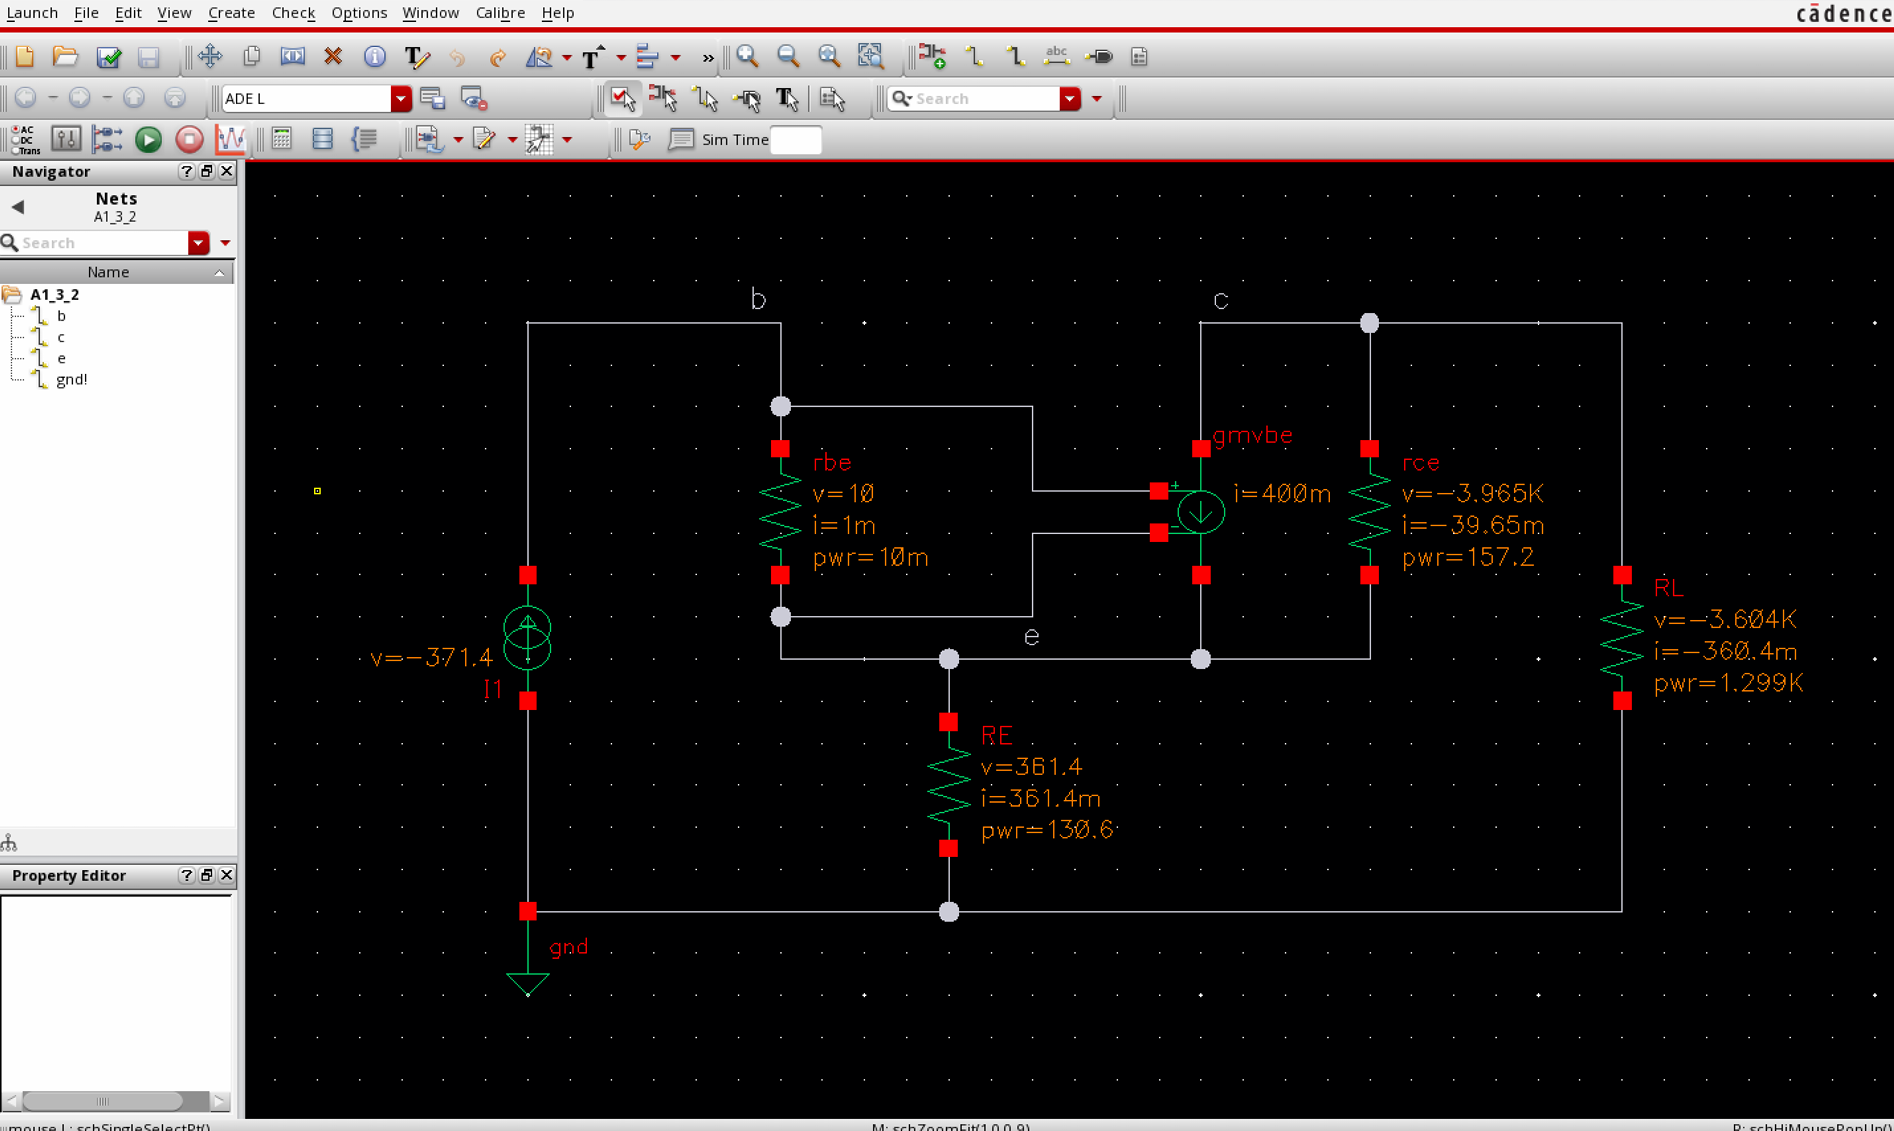
\includegraphics[width=1\textwidth]{chapters/figure/A4/A4input.png}
\caption{输入电阻仿真结果}
\label{输入电阻仿真结果}
\end{figure}

\tt{给恒流源加1mA电流，仿真得到输入电阻为$R_{in}=371.4k\Omega$，与理论计算结果一致}

\subsection{输出电阻：}

\begin{figure}[H]
\centering
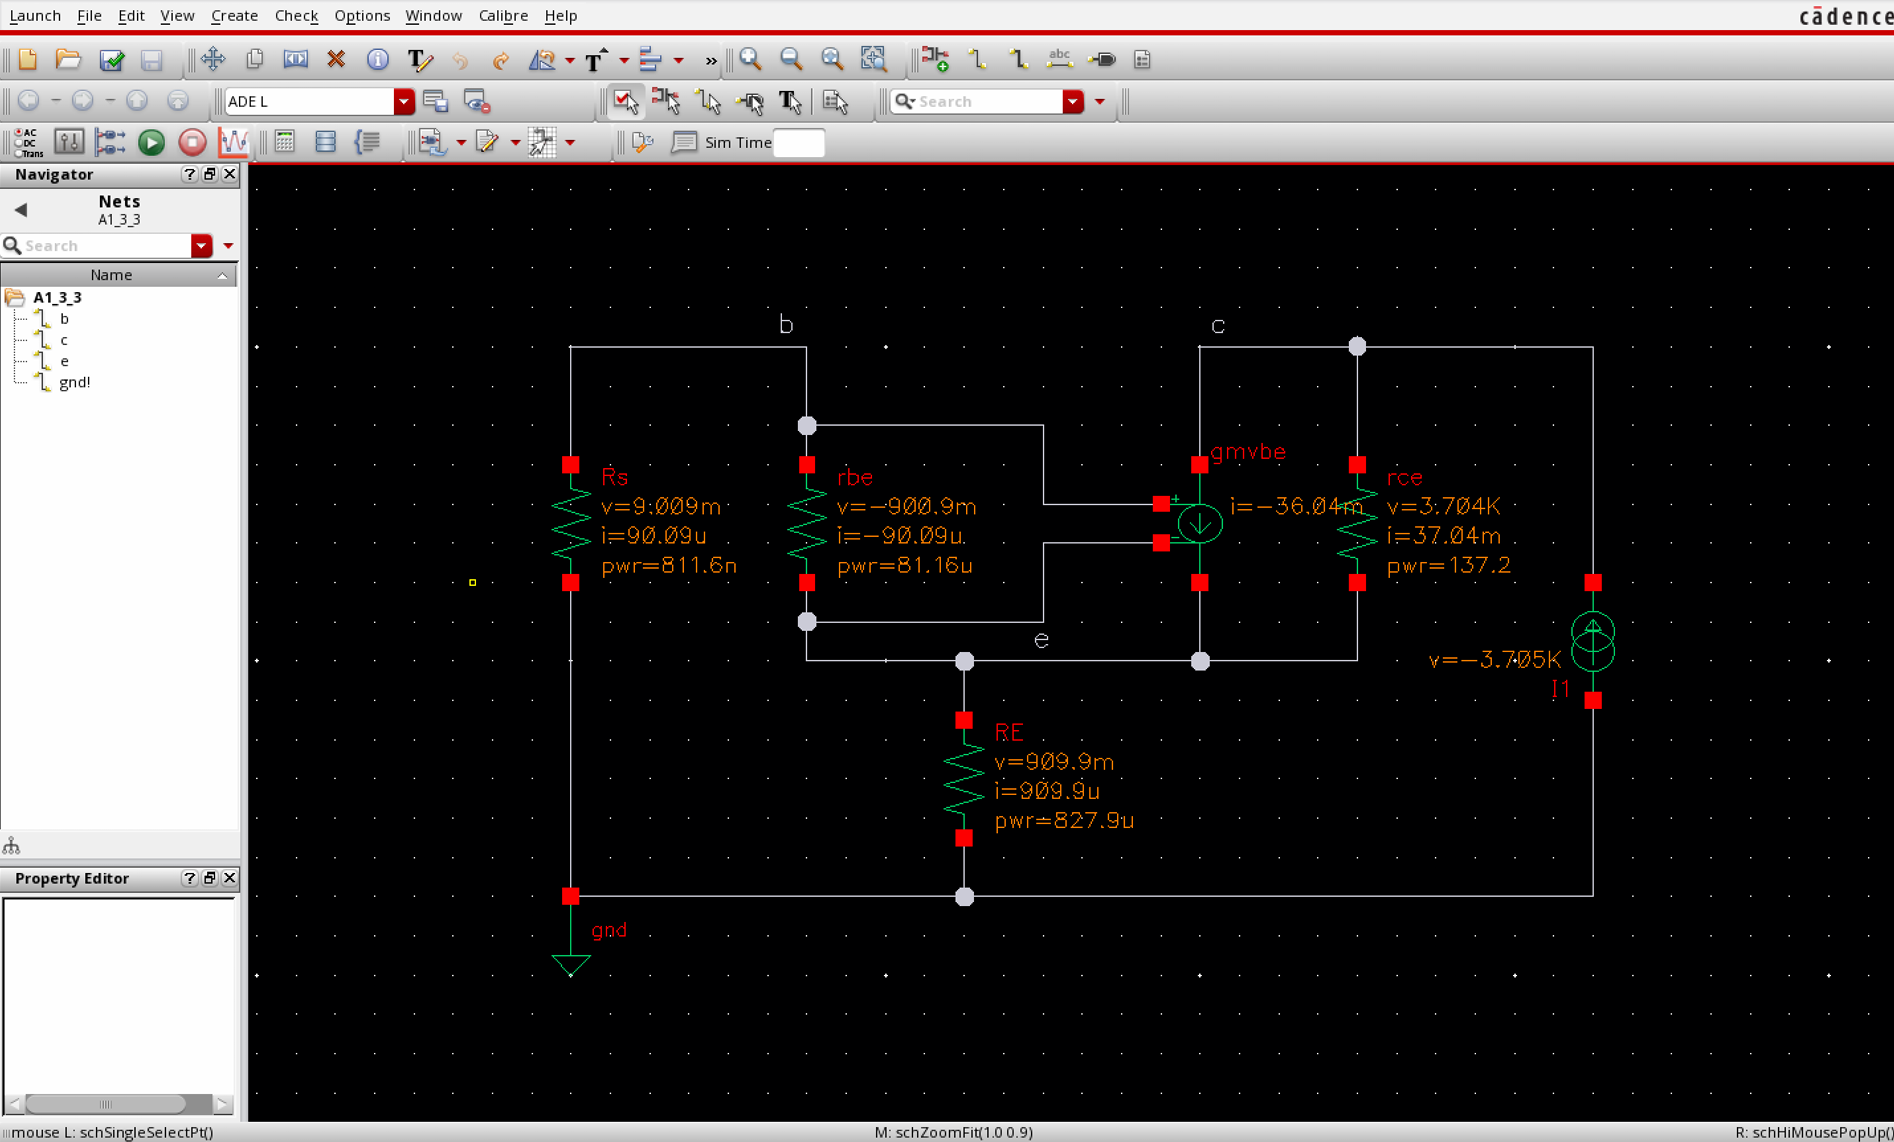
\includegraphics[width=1\textwidth]{chapters/figure/A4/A4output.png}
\caption{输出电阻仿真结果}
\label{输出电阻仿真结果}
\end{figure}

\tt{给恒流源加1mA电流，仿真得到输出电阻为$R_{out}=3.705M\Omega$，与理论计算结果一致}

\subsection{电压放大倍数：}

\begin{figure}[H]
\centering
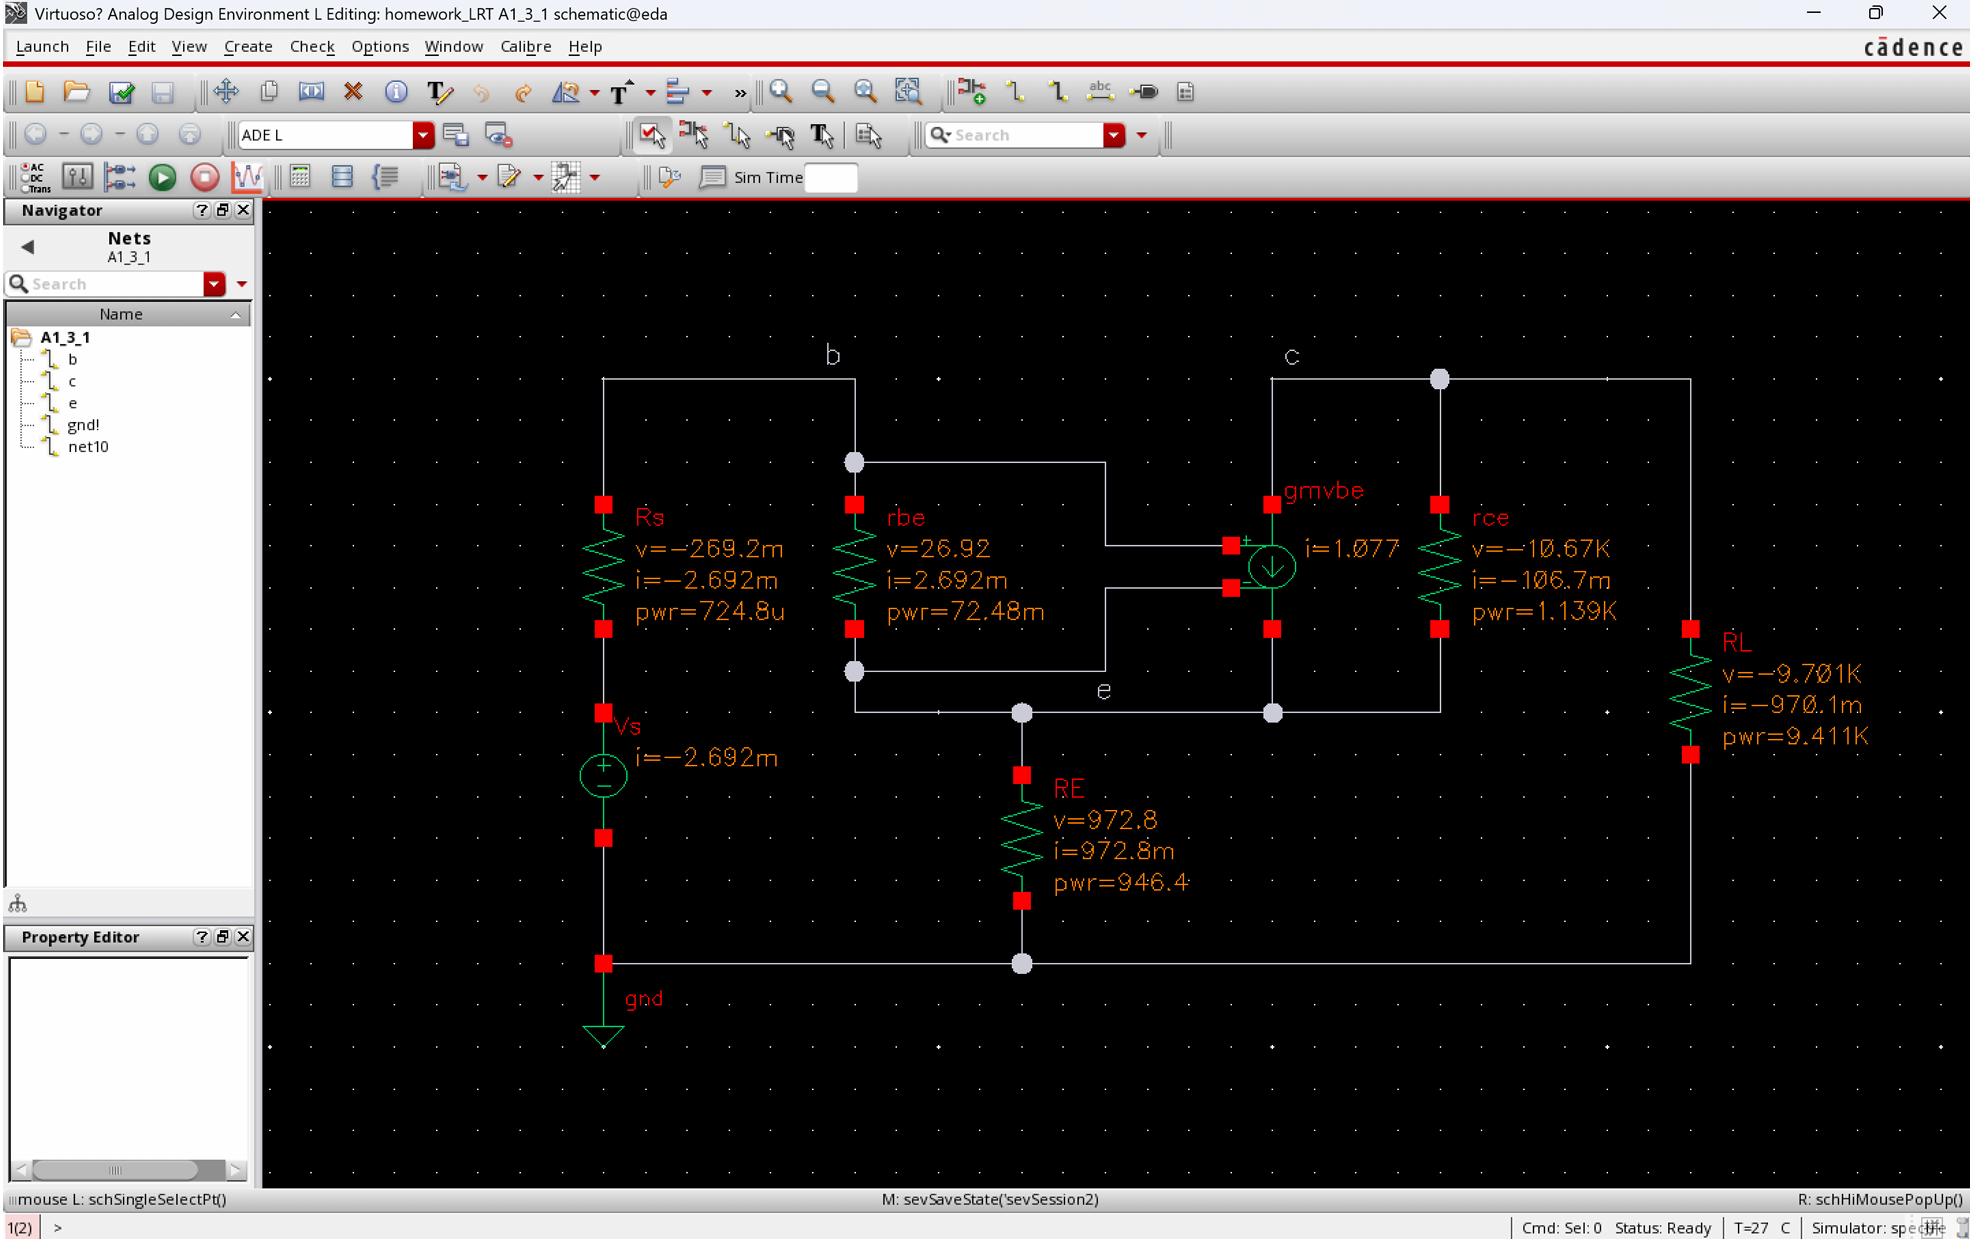
\includegraphics[width=1\textwidth]{chapters/figure/A4/A4AV.png}
\caption{电压放大倍数仿真结果}
\label{电压放大倍数仿真结果}
\end{figure}

\tt{$V_{s}=1kV$,$V_{L}=-9.701kV$，仿真得到电压放大倍数为$A_v=-9.701$，与理论计算结果一致}

\subsection{等效诺顿电流源：}

\begin{figure}[H]
\centering
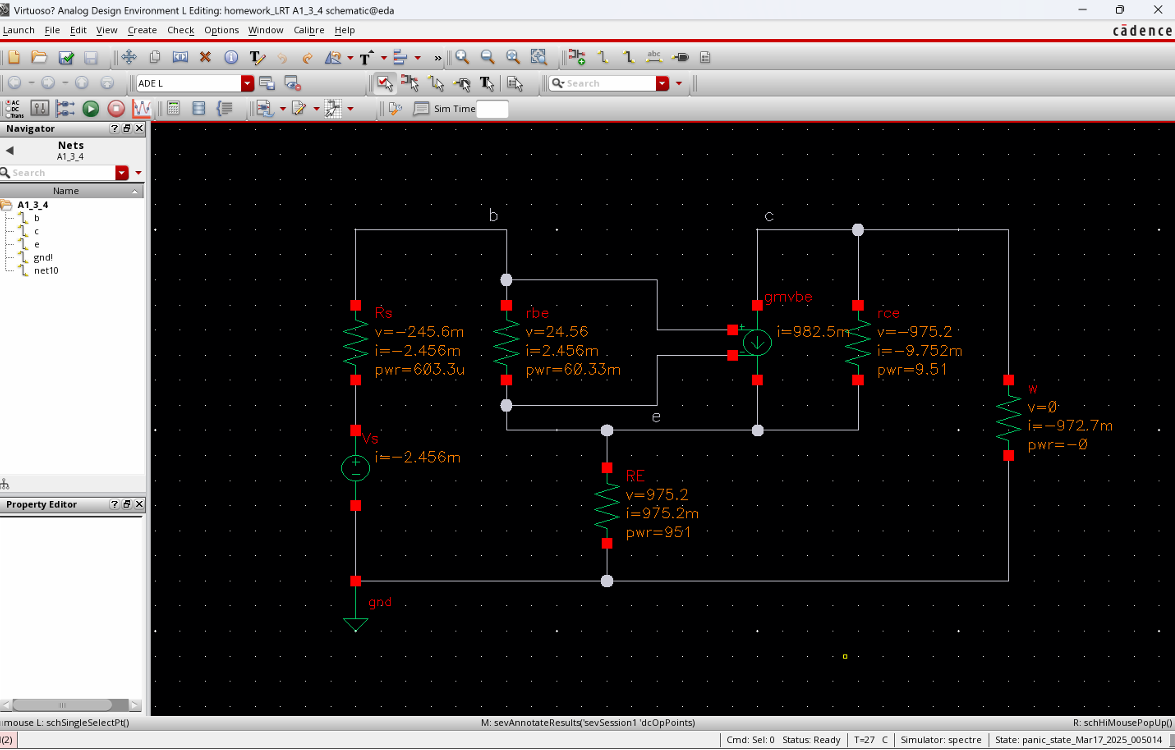
\includegraphics[width=1\textwidth]{chapters/figure/A4/A4IN.png}
\caption{等效诺顿电流源仿真结果}
\label{等效诺顿电流源仿真结果}
\end{figure}

\tt{$V_{s}=1kV$,$I_{N}=-972.7mA$，仿真得到等效诺顿电流源为$I_N=-972.7uS$，与理论计算结果一致}

\myendpage

\end{document}